\chapter{La composition graphique}
\section*{Introduction du chapitre}
\addcontentsline{toc}{section}{Introduction du chapitre}

Dans le chapitre précédent, nous avons défini le design graphique, retracé son histoire, exploré ses domaines et décrit le processus de création. Tout cela constitue le cadre général du métier. Mais il arrive un moment où il faut entrer dans le vif du sujet : comment organise-t-on concrètement les éléments visuels pour produire un message efficace ?

C'est l'objet de ce chapitre. La composition graphique est le cœur du métier de designer. C'est elle qui transforme un ensemble d'éléments épars (texte, image, couleur, forme) en un tout cohérent, lisible, harmonieux et signifiant. Sans composition, il n'y a que des éléments juxtaposés. Avec la composition, il y a un message.

Ce chapitre est sans doute le plus important de la première partie de ta formation. Les principes que tu vas apprendre ici te serviront dans tous les projets, quel que soit le logiciel utilisé, quel que soit le support, quel que soit le domaine. Photoshop, Illustrator, InDesign : tous ces outils ne sont que des instruments au service de la composition. Si tu maîtrises la composition, tu pourras t'adapter à n'importe quel outil. Si tu ne la maîtrises pas, aucun logiciel ne pourra compenser.

Nous allons procéder progressivement. D'abord, nous définirons ce qu'est la composition graphique. Ensuite, nous examinerons les éléments fondamentaux du langage visuel. Puis, nous étudierons les principes qui régissent l'organisation de ces éléments : équilibre, hiérarchie, alignement, contraste, proximité, répétition, espace négatif. Enfin, nous verrons comment utiliser les grilles de composition et comment éviter les erreurs courantes.

Prends le temps de bien assimiler chaque section. La composition est une compétence qui se construit par la pratique, mais elle repose sur des principes théoriques qu'il faut d'abord comprendre. Ne brûle pas les étapes.

%==================================================
\section{Définition de la composition graphique}

\subsection{Qu'est-ce que la composition graphique ?}

La composition graphique est l'organisation réfléchie et intentionnelle des éléments visuels (texte, image, forme, couleur) dans un espace donné, en vue de produire un message clair, lisible, harmonieux et efficace.

Cette définition mérite d'être décomposée terme par terme.

\subsubsection{« Organisation réfléchie et intentionnelle »}

La composition n'est pas un acte spontané ou aléatoire. Elle est réfléchie (on pense avant d'agir) et intentionnelle (on agit dans un but précis). Chaque élément est placé à un endroit précis, pour une raison précise. Rien n'est laissé au hasard.

Cela ne signifie pas que la composition ne laisse aucune place à l'intuition ou à l'expérimentation. Mais même l'expérimentation doit être consciente : on essaie quelque chose, on observe le résultat, on ajuste. La composition est un processus d'essais, d'erreurs et de corrections.

\subsubsection{« Des éléments visuels »}

Les éléments visuels sont les briques de la composition. On les appelle parfois les éléments du langage visuel. Ils comprennent :
\begin{itemize}
  \item Le texte (titres, sous-titres, paragraphes, légendes).
  \item Les images (photographies, illustrations, pictogrammes).
  \item Les formes (rectangles, cercles, lignes, tracés).
  \item Les couleurs (teintes, valeurs, saturations).
  \item Les textures (matières, motifs, grains).
\end{itemize}

Nous détaillerons ces éléments dans la section suivante.

\subsubsection{« Dans un espace donné »}

Toute composition s'inscrit dans un espace délimité : une feuille de papier, un écran, une affiche, un emballage. Cet espace a des dimensions, des proportions, une orientation. Il impose des contraintes : on ne compose pas de la même manière pour un format carré, un format paysage ou un format portrait.

L'espace de composition est parfois appelé cadre ou format. C'est le contenant dans lequel les éléments sont organisés.

\subsubsection{« En vue de produire un message »}

La composition n'est pas une fin en soi : elle est au service d'un message. Elle doit rendre ce message :
\begin{itemize}
  \item \textbf{Clair} : compréhensible immédiatement.
  \item \textbf{Lisible} : accessible sans effort.
  \item \textbf{Harmonieux} : agréable à regarder.
  \item \textbf{Efficace} : atteint son objectif (informer, séduire, convaincre).
\end{itemize}

Une composition réussie est une composition qui fonctionne : le spectateur comprend ce qu'on veut lui dire, et il le comprend rapidement.

\subsection{Composition et mise en page : quelle différence ?}

Les termes « composition » et « mise en page » sont souvent utilisés de manière interchangeable. Il existe cependant une nuance :
\begin{itemize}
  \item La \textbf{composition} est un terme plus large : elle désigne l'organisation de tous les éléments visuels, y compris dans des contextes non éditoriaux (affiche, logo, packaging).
  \item La \textbf{mise en page} est un terme plus spécifique : elle désigne l'organisation des éléments dans un document éditorial (livre, magazine, rapport), avec une attention particulière au texte et à sa disposition.
\end{itemize}

Dans la pratique, les deux termes se recoupent largement. Nous utiliserons « composition » comme terme général.

\subsection{Pourquoi la composition est-elle essentielle ?}

La composition est essentielle pour plusieurs raisons.

\subsubsection{Elle guide le regard}

Le spectateur ne regarde pas une image de manière aléatoire. Son œil est attiré par certains éléments, puis circule dans la composition selon un parcours plus ou moins prévisible. La composition oriente ce parcours : elle décide ce qui sera vu en premier, en deuxième, en troisième.

Une composition réussie crée un parcours visuel fluide, qui mène le spectateur de l'information principale aux informations secondaires, sans le perdre.

\subsubsection{Elle hiérarchise l'information}

Toute information n'a pas la même importance. La composition hiérarchise : elle distingue le message principal, les messages secondaires, les informations pratiques. Sans hiérarchie, tout est au même niveau, et rien n'émerge.

\subsubsection{Elle crée de l'harmonie}

Une composition réussie est harmonieuse : les éléments semblent être à leur place, les proportions sont équilibrées, les couleurs s'accordent. Cette harmonie n'est pas seulement esthétique : elle renforce la crédibilité du message. Un visuel harmonieux inspire confiance ; un visuel désordonné inspire le doute.

\subsubsection{Elle facilite la mémorisation}

Une composition claire et hiérarchisée est plus mémorisable qu'une composition confuse. Le cerveau retient mieux ce qu'il comprend facilement.

\subsubsection{Elle distingue le professionnel de l'amateur}

La composition est l'un des principaux critères qui distinguent un visuel professionnel d'un visuel amateur. Un amateur va « remplir » un espace avec des éléments, sans réfléchir à leur organisation. Un professionnel va « construire » un espace, en organisant chaque élément en fonction d'un objectif.

\subsection{Les trois niveaux de la composition}

On peut distinguer trois niveaux dans la composition graphique :

\subsubsection{Le niveau macroscopique : la structure globale}

C'est l'organisation d'ensemble de la composition : la répartition des masses, les grands blocs (texte, image), les zones de respiration. C'est ce qu'on perçoit au premier coup d'œil, avant même de lire le contenu.

\subsubsection{Le niveau mésoscopique : les relations entre éléments}

C'est l'organisation des relations entre les éléments : alignements, proximités, contrastes, répétitions. C'est ce qu'on perçoit en observant la composition pendant quelques secondes.

\subsubsection{Le niveau microscopique : les détails}

C'est l'organisation des détails : espacements entre les lettres, interlignage, position exacte des éléments, épaisseur des traits. C'est ce qu'on perçoit en observant attentivement, parfois avec une loupe.

Les trois niveaux sont interdépendants. Une composition peut avoir une bonne structure globale mais des détails mal soignés. Elle peut avoir des détails soignés mais une structure confuse. Une composition professionnelle soigne les trois niveaux.

\subsection{Les grands principes de la composition}

La composition graphique repose sur un certain nombre de principes fondamentaux. Ces principes sont parfois appelés principes de design ou principes de Gestalt. Ils ont été formulés par des psychologues de la perception au début du XX\textsuperscript{e} siècle, puis adoptés et adaptés par les designers.

Voici les principaux principes que nous étudierons dans ce chapitre :
\begin{enumerate}
  \item \textbf{Équilibre} : répartition harmonieuse des masses visuelles.
  \item \textbf{Hiérarchie} : ordre d'importance des éléments.
  \item \textbf{Alignement} : relations visuelles entre les éléments.
  \item \textbf{Contraste} : mise en évidence par la différence.
  \item \textbf{Proximité} : regroupement des éléments liés.
  \item \textbf{Répétition} : création de rythme et de cohérence.
  \item \textbf{Espace négatif} : utilisation de l'espace vide.
  \item \textbf{Grille} : structure sous-jacente de la composition.
\end{enumerate}

Chacun de ces principes fera l'objet d'une section détaillée dans ce chapitre.

\subsection{Les lois de la Gestalt}

Avant d'aller plus loin, il est utile de dire quelques mots sur la Gestalt (« forme », en allemand). La Gestalt est un courant de psychologie né en Allemagne au début du XX\textsuperscript{e} siècle (Wertheimer, Koffka, Köhler). Elle étudie la manière dont le cerveau perçoit les formes et organise les informations visuelles.

Les lois de la Gestalt sont fondamentales pour comprendre la composition graphique. Voici les principales :

\subsubsection{Loi de proximité}

Les éléments proches les uns des autres sont perçus comme appartenant à un même groupe.

\subsubsection{Loi de similitude}

Les éléments qui se ressemblent (forme, couleur, taille) sont perçus comme appartenant à un même groupe.

\subsubsection{Loi de continuité}

Les éléments alignés ou qui suivent une direction continue sont perçus comme appartenant à un même ensemble.

\subsubsection{Loi de fermeture}

Le cerveau tend à compléter les formes incomplètes pour les percevoir comme des ensembles fermés.

\subsubsection{Loi de figure-fond}

Le cerveau distingue spontanément une figure (ce qui est au premier plan) d'un fond (ce qui est à l'arrière-plan).

\begin{figure}[ht]
\centering
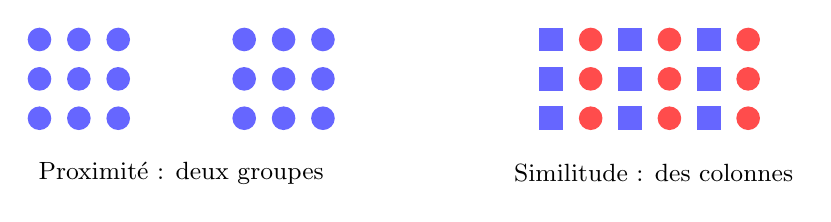
\begin{tikzpicture}
% proximité : deux groupes
\foreach \x in {0,1,2} \foreach \y in {0,1,2}{
  \fill[blue!60] (\x*0.5,\y*0.5) circle(0.15);
  \fill[blue!60] (\x*0.5+2.6,\y*0.5) circle(0.15);}
\node[font=\small] at (1.8,-0.7) {Proximité : deux groupes};
% similitude : colonnes alternées
\foreach \x in {0,...,5} \foreach \y in {0,1,2}{
  \ifodd\x \fill[red!70] (\x*0.5+6.5,\y*0.5) circle(0.15);
  \else \fill[blue!60] (\x*0.5+6.35,\y*0.5-0.15) rectangle ++(0.3,0.3);\fi}
\node[font=\small] at (7.8,-0.7) {Similitude : des colonnes};
\end{tikzpicture}
\caption{Deux lois de la Gestalt : le rapprochement crée des groupes, la ressemblance crée des familles.}
\end{figure}

\subsubsection{Loi de destin commun}

Les éléments qui se déplacent ou évoluent dans la même direction sont perçus comme appartenant à un même groupe.

Ces lois expliquent pourquoi certaines compositions « fonctionnent » et d'autres non. Elles sont la base scientifique de la composition graphique.

\subsection{Ce qu'il faut retenir de cette section}

\begin{retenir}
\begin{itemize}
  \item La composition graphique est l'organisation réfléchie et intentionnelle des éléments visuels dans un espace donné.
  \item Elle vise à produire un message clair, lisible, harmonieux et efficace.
  \item Elle guide le regard, hiérarchise l'information, crée de l'harmonie, facilite la mémorisation.
  \item Elle distingue le professionnel de l'amateur.
  \item Elle repose sur des principes (équilibre, hiérarchie, alignement, contraste, proximité, répétition, espace négatif, grille).
  \item Elle s'appuie sur les lois de la Gestalt (proximité, similitude, continuité, fermeture, figure-fond, destin commun).
\end{itemize}
\end{retenir}

Maintenant que nous avons défini la composition graphique, nous allons examiner, dans la section suivante, les éléments fondamentaux du langage visuel. Quels sont les matériaux de base avec lesquels le designer compose ? Comment les reconnaître, les distinguer, les utiliser ? C'est ce que nous allons voir.

%==================================================
\section{Les éléments fondamentaux du langage visuel}

\subsection{Le langage visuel : une analogie avec le langage écrit}

Pour comprendre les éléments du langage visuel, on peut faire une analogie avec le langage écrit. En français, on distingue :
\begin{itemize}
  \item Les lettres (a, b, c\ldots) : les unités de base.
  \item Les mots (chat, maison\ldots) : des assemblages de lettres porteurs de sens.
  \item Les phrases : des assemblages de mots porteurs d'un sens complet.
  \item Les paragraphes : des assemblages de phrases organisés autour d'une idée.
  \item Le texte : un ensemble de paragraphes formant un message.
\end{itemize}

En design graphique, on distingue de manière analogue :
\begin{itemize}
  \item Les éléments de base : point, ligne, forme, couleur, texture.
  \item Les unités visuelles : un titre, une image, un pictogramme.
  \item Les groupes : un bloc de texte, une série d'images.
  \item La composition : l'ensemble organisé.
\end{itemize}

Cette analogie n'est pas parfaite, mais elle aide à comprendre que la composition graphique est un langage, avec sa grammaire et sa syntaxe.

\subsection{Les éléments de base du langage visuel}

Les éléments de base du langage visuel sont au nombre de cinq :
\begin{enumerate}
  \item Le point.
  \item La ligne.
  \item La forme.
  \item La couleur.
  \item La texture.
\end{enumerate}

Nous allons les examiner un par un.

\subsubsection{Le point}

\textbf{Définition :} le point est l'élément visuel le plus petit et le plus simple. Il n'a ni longueur ni largeur significative : il marque une position dans l'espace.

\textbf{Rôle dans la composition :}
\begin{itemize}
  \item Attirer l'attention : un point isolé attire le regard.
  \item Créer un rythme : une série de points crée un rythme visuel.
  \item Structurer : les points peuvent servir de repères, de puces, de séparateurs.
  \item Suggérer : un point peut suggérer un élément (un œil, une étoile, une puce).
\end{itemize}

\textbf{Exemples :}
\begin{itemize}
  \item Les puces dans une liste.
  \item Les points sur un i.
  \item Les points de suspension.
  \item Les pixels d'une image.
\end{itemize}

\textbf{Dans la composition :} le point est rarement utilisé seul. Il est souvent combiné avec d'autres éléments. Mais il peut jouer un rôle important : un point bien placé peut équilibrer une composition, attirer l'attention sur un détail, créer un contraste.

\subsubsection{La ligne}

\textbf{Définition :} la ligne est une succession de points. Elle a une longueur, une direction, une épaisseur. Elle peut être droite, courbe, brisée, continue, discontinue.

\textbf{Rôle dans la composition :}
\begin{itemize}
  \item Délimiter : une ligne peut séparer deux zones, encadrer un élément.
  \item Guider : une ligne peut conduire le regard dans une direction.
  \item Relier : une ligne peut relier deux éléments.
  \item Suggérer : une ligne peut suggérer un mouvement, une tension, une émotion.
  \item Structurer : les lignes peuvent servir de base à une grille.
\end{itemize}

\textbf{Types de lignes :}
\begin{itemize}
  \item Ligne droite : rigueur, stabilité, ordre.
  \item Ligne courbe : douceur, fluidité, mouvement.
  \item Ligne brisée : énergie, tension, dynamisme.
  \item Ligne épaisse : force, présence.
  \item Ligne fine : délicatesse, élégance.
  \item Ligne continue : unité, cohérence.
  \item Ligne discontinue : fragmentation, suggestion.
\end{itemize}

\textbf{Exemples :}
\begin{itemize}
  \item Les filets de séparation dans un journal.
  \item Les soulignements.
  \item Les flèches.
  \item Les contours de formes.
\end{itemize}

\textbf{Dans la composition :} la ligne est un élément omniprésent. Elle structure, guide, délimite. Les lignes implicites (alignements) sont aussi importantes que les lignes explicites.

\subsubsection{La forme}

\textbf{Définition :} la forme est une surface délimitée par un contour. Elle a une longueur, une largeur, une silhouette. Elle peut être géométrique (carré, cercle, triangle) ou organique (libre, irrégulière).

\textbf{Rôle dans la composition :}
\begin{itemize}
  \item Structurer : les formes créent la structure de la composition.
  \item Attirer : les formes attirent le regard.
  \item Signifier : certaines formes ont une signification symbolique (carré = stabilité, cercle = harmonie, triangle = dynamisme).
  \item Contenir : les formes peuvent contenir du texte ou des images.
\end{itemize}

\textbf{Types de formes :}
\begin{itemize}
  \item Formes géométriques : carré, rectangle, cercle, triangle, polygone.
  \item Formes organiques : formes libres, irrégulières, naturelles.
  \item Formes abstraites : formes non figuratives.
  \item Formes figuratives : formes représentant des objets ou des êtres.
\end{itemize}

\textbf{Exemples :}
\begin{itemize}
  \item Les cadres.
  \item Les pastilles de couleur.
  \item Les pictogrammes.
  \item Les blocs de texte.
\end{itemize}

\textbf{Dans la composition :} les formes sont les éléments structurants de la composition. Elles définissent les zones, les blocs, les masses.

\subsubsection{La couleur}

\textbf{Définition :} la couleur est la sensation produite par la lumière réfléchie par un objet. Elle a trois dimensions : la teinte (la couleur elle-même), la saturation (l'intensité), la luminosité (la clarté).

\textbf{Rôle dans la composition :}
\begin{itemize}
  \item Attirer : les couleurs vives attirent le regard.
  \item Hiérarchiser : les couleurs peuvent distinguer les niveaux d'information.
  \item Émouvoir : les couleurs suscitent des émotions.
  \item Signifier : les couleurs ont des significations culturelles (rouge = danger, vert = nature).
  \item Structurer : les couleurs peuvent délimiter des zones, créer des ensembles.
\end{itemize}

Nous étudierons la couleur en détail dans le chapitre 3. Pour l'instant, retiens qu'elle est un élément fondamental de la composition.

\textbf{Exemples :}
\begin{itemize}
  \item Les fonds de couleur.
  \item Les aplats.
  \item Les dégradés.
  \item Les contrastes de couleur.
\end{itemize}

\textbf{Dans la composition :} la couleur est un élément puissant. Elle peut unifier ou fragmenter, attirer ou repousser, apaiser ou dynamiser.

\subsubsection{La texture}

\textbf{Définition :} la texture est la qualité de surface d'un élément. Elle peut être visuelle (perçue par l'œil) ou tactile (perçue par le toucher). Elle peut être lisse, rugueuse, granuleuse, veloutée.

\textbf{Rôle dans la composition :}
\begin{itemize}
  \item Enrichir : la texture ajoute de la richesse visuelle.
  \item Différencier : la texture distingue des zones.
  \item Évoquer : la texture évoque des matières, des ambiances.
  \item Attirer : la texture attire le regard.
\end{itemize}

\textbf{Types de textures :}
\begin{itemize}
  \item Textures naturelles : bois, pierre, tissu.
  \item Textures artificielles : plastique, métal, verre.
  \item Textures graphiques : motifs, trames, grains.
\end{itemize}

\textbf{Exemples :}
\begin{itemize}
  \item Les fonds texturés.
  \item Les motifs répétés.
  \item Les images de matière.
\end{itemize}

\textbf{Dans la composition :} la texture est souvent utilisée avec modération. Trop de textures créent de la confusion. Mais bien utilisée, elle enrichit la composition.

\subsection{Les éléments de composition : les unités visuelles}

Au-delà des éléments de base, la composition graphique utilise des unités visuelles plus complexes :

\subsubsection{Le texte}

Le texte est l'unité visuelle qui porte le message verbal. Il peut prendre plusieurs formes :
\begin{itemize}
  \item Titre : le texte principal, le plus grand, le plus visible.
  \item Sous-titre : un texte secondaire, qui complète le titre.
  \item Paragraphe : un bloc de texte courant.
  \item Légende : un texte qui accompagne une image.
  \item Mention : un texte technique (date, lieu, prix).
\end{itemize}

Le texte a des propriétés visuelles : taille, graisse, couleur, alignement, interlignage. Ces propriétés déterminent sa lisibilité et sa hiérarchie.

\subsubsection{L'image}

L'image est l'unité visuelle qui porte le message visuel non verbal. Elle peut être :
\begin{itemize}
  \item Photographie : une image du réel.
  \item Illustration : une image créée.
  \item Pictogramme : une image simplifiée, symbolique.
  \item Graphique : une représentation de données.
\end{itemize}

L'image a des propriétés visuelles : cadrage, échelle, contraste, couleur. Ces propriétés déterminent son impact et sa signification.

\subsubsection{Le bloc}

Le bloc est un ensemble d'éléments traités comme une unité. Par exemple :
\begin{itemize}
  \item Un bloc de texte.
  \item Un bloc d'images.
  \item Un bloc d'informations.
\end{itemize}

Les blocs sont des unités de composition. Ils permettent de structurer la composition en zones distinctes.

\subsubsection{Le groupe}

Le groupe est un ensemble d'éléments qui vont ensemble. Par exemple :
\begin{itemize}
  \item Un logo et son slogan.
  \item Une image et sa légende.
  \item Une série de pictogrammes.
\end{itemize}

Les groupes sont perçus comme des unités par les lois de la Gestalt (proximité, similitude).

\subsection{Les relations entre les éléments}

La composition ne consiste pas seulement à placer des éléments : elle consiste à créer des relations entre eux. Ces relations sont de plusieurs types :

\subsubsection{Relations de proximité}

Les éléments proches sont perçus comme liés. Les éléments éloignés sont perçus comme séparés.

\subsubsection{Relations d'alignement}

Les éléments alignés sont perçus comme liés. Les éléments désalignés sont perçus comme séparés.

\subsubsection{Relations de similitude}

Les éléments qui se ressemblent (couleur, forme, taille) sont perçus comme liés.

\subsubsection{Relations de contraste}

Les éléments qui diffèrent sont perçus comme distincts. Le contraste attire l'attention.

\subsubsection{Relations de hiérarchie}

Les éléments ont des niveaux d'importance différents. La hiérarchie organise la lecture.

Ces relations sont la matière première de la composition. Le designer les utilise pour construire le message.

\subsection{Ce qu'il faut retenir de cette section}

\begin{retenir}
\begin{itemize}
  \item Les éléments de base du langage visuel sont : le point, la ligne, la forme, la couleur, la texture.
  \item Les unités visuelles sont le texte, l'image, le bloc et le groupe.
  \item Les relations entre éléments (proximité, alignement, similitude, contraste, hiérarchie) sont la matière première de la composition.
\end{itemize}
\end{retenir}

\begin{astuce}
Quand une composition te semble confuse, retire un élément à la fois. Si le message reste lisible sans lui, cet élément n'avait pas de fonction.
\end{astuce}

%==================================================
\section{Les principes de l'équilibre visuel}

\subsection{Qu'est-ce que l'équilibre visuel ?}

L'\terme{équilibre visuel} est la sensation de stabilité que procure une composition. Chaque élément possède un \terme{poids visuel} : plus il est grand, sombre, saturé, complexe ou isolé, plus il pèse. Une composition est équilibrée lorsque les poids sont répartis de manière à ce que le regard ne soit pas tiré d'un seul côté.

Imagine une balance : le centre de la page est le point d'appui. Un gros bloc sombre à gauche doit être compensé, à droite, par autre chose : un élément plus petit mais plus éloigné du centre, ou plus contrasté.

\subsection{Les facteurs qui déterminent le poids visuel}

\begin{table}[h!]
\centering
\begin{tabular}{@{}p{3.5cm}p{5cm}p{5cm}@{}}
\toprule
\textbf{Facteur} & \textbf{Poids fort} & \textbf{Poids faible} \\
\midrule
Taille & Grand élément & Petit élément \\
Valeur & Élément sombre sur fond clair & Élément clair sur fond clair \\
Saturation & Couleur vive & Couleur pâle ou grisée \\
Complexité & Détails nombreux & Forme simple \\
Position & Éloigné du centre & Proche du centre \\
Isolement & Élément seul dans un espace vide & Élément noyé dans un groupe \\
\bottomrule
\end{tabular}
\caption{Les facteurs du poids visuel.}
\end{table}

\subsection{Les trois types d'équilibre}

\subsubsection{L'équilibre symétrique}

Les éléments sont répartis de manière identique de part et d'autre d'un axe (le plus souvent vertical). L'effet est stable, solennel, formel. On le rencontre dans les invitations officielles, les logos institutionnels, les couvertures de livres classiques.

\subsubsection{L'équilibre asymétrique}

Les éléments sont différents de part et d'autre de l'axe, mais leurs poids se compensent. L'effet est plus dynamique, plus moderne, plus subtil. Il est plus difficile à réussir mais offre plus de liberté.

\subsubsection{L'équilibre radial}

Les éléments rayonnent à partir d'un point central, comme les pétales d'une fleur ou les rayons d'une roue. L'effet attire le regard vers le centre. On le retrouve dans les mandalas, les rosaces, certains logos circulaires.

\begin{figure}[ht]
\centering
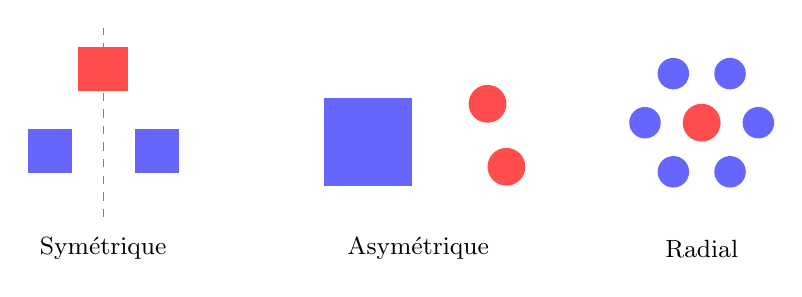
\begin{tikzpicture}[scale=0.8]
% symétrique
\draw[gray,dashed] (1.5,-0.2) -- (1.5,2.8);
\fill[blue!60] (0.3,0.5) rectangle (1,1.2);
\fill[blue!60] (2,0.5) rectangle (2.7,1.2);
\fill[red!70] (1.1,1.8) rectangle (1.9,2.5);
\node[font=\small] at (1.5,-0.7) {Symétrique};
% asymétrique
\fill[blue!60] (5,0.3) rectangle (6.4,1.7);
\fill[red!70] (7.6,1.6) circle(0.3);
\fill[red!70] (7.9,0.6) circle(0.3);
\node[font=\small] at (6.5,-0.7) {Asymétrique};
% radial
\foreach \a in {0,60,...,300}{\fill[blue!60] (11,1.3) ++(\a:0.9) circle(0.25);}
\fill[red!70] (11,1.3) circle(0.3);
\node[font=\small] at (11,-0.7) {Radial};
\end{tikzpicture}
\caption{Les trois types d'équilibre visuel.}
\end{figure}

\begin{astuce}
Pour tester l'équilibre d'une composition, plisse les yeux ou floute-la : il ne reste que des masses. Si l'ensemble penche d'un côté, redistribue les poids.
\end{astuce}

\subsection{Étude de cas : la page d'accueil de Google}

La page d'accueil du moteur de recherche Google est un exemple d'équilibre symétrique très épuré : un logo centré, un champ de recherche centré en dessous, et très peu d'autres éléments. L'axe central structure tout, et l'espace vide autour concentre l'attention sur l'action unique attendue de l'utilisateur : chercher.

\begin{retenir}
\begin{itemize}
  \item Chaque élément a un poids visuel (taille, valeur, saturation, complexité, position, isolement).
  \item L'équilibre peut être symétrique, asymétrique ou radial.
  \item L'asymétrie est plus dynamique mais demande de compenser les poids.
\end{itemize}
\end{retenir}

%==================================================
\section{La hiérarchie visuelle}

\subsection{Définition}

La \terme{hiérarchie visuelle} est l'organisation des éléments selon leur ordre d'importance. Elle répond à une question simple : que doit voir le lecteur en premier, en deuxième, en troisième ?

\begin{defbox}[Définition : niveaux de lecture]
On distingue généralement trois niveaux : le \terme{niveau primaire} (ce qu'on voit en premier : titre, image principale), le \terme{niveau secondaire} (sous-titres, informations clés) et le \terme{niveau tertiaire} (détails, mentions, légendes).
\end{defbox}

\subsection{Les outils de la hiérarchie}

\begin{table}[h!]
\centering
\begin{tabular}{@{}p{3.5cm}p{10.5cm}@{}}
\toprule
\textbf{Outil} & \textbf{Effet} \\
\midrule
Taille & Le plus grand est lu en premier. \\
Contraste de valeur & Un élément très sombre ou très clair sur son fond ressort. \\
Couleur & Une couleur vive ou inattendue attire le regard. \\
Graisse & Le gras domine le maigre. \\
Position & Le haut et la gauche sont généralement lus en premier (dans une culture de lecture de gauche à droite). \\
Espace autour & Un élément isolé gagne de l'importance. \\
\bottomrule
\end{tabular}
\caption{Les principaux outils de la hiérarchie visuelle.}
\end{table}

\subsection{Les parcours de lecture}

Le regard suit rarement un chemin au hasard. Dans les cultures qui lisent de gauche à droite, on décrit souvent des parcours en \terme{Z} (pages peu denses, affiches) ou en \terme{F} (pages très textuelles, pages web). Ces schémas sont des tendances, pas des lois : une hiérarchie forte les surpasse.

\subsection{Les erreurs de hiérarchie}

\begin{erreur}
Tout mettre en gras, en grand ou en couleur : quand tout est important, rien ne l'est. Une bonne hiérarchie suppose que certains éléments soient volontairement discrets.
\end{erreur}

\subsection{Étude de cas : une affiche de film}

Sur une affiche de cinéma, le niveau primaire est le plus souvent l'image (visage, scène) et le titre ; le niveau secondaire porte les noms des acteurs ; le niveau tertiaire regroupe, en petits caractères en bas, le générique technique. Cette organisation est reprise très fréquemment car elle correspond à l'ordre d'intérêt du public.

\begin{retenir}
\begin{itemize}
  \item La hiérarchie ordonne la lecture en trois niveaux : primaire, secondaire, tertiaire.
  \item Ses outils : taille, contraste, couleur, graisse, position, espace.
  \item Trop d'éléments mis en avant détruisent la hiérarchie.
\end{itemize}
\end{retenir}

%==================================================
\section{L'alignement des éléments}

\subsection{Pourquoi aligner ?}

L'\terme{alignement} consiste à placer les éléments le long de lignes communes, visibles ou invisibles. Il crée des relations entre des éléments éloignés, donne une impression d'ordre et de rigueur, et facilite la lecture. Une composition où rien n'est aligné paraît instable, même si chaque élément est soigné.

\subsection{Les types d'alignement}

\begin{table}[h!]
\centering
\begin{tabular}{@{}p{3.2cm}p{4.5cm}p{6.3cm}@{}}
\toprule
\textbf{Alignement} & \textbf{Caractéristique} & \textbf{Usage courant} \\
\midrule
À gauche & Bord gauche net, bord droit irrégulier & Texte courant, très lisible \\
À droite & Bord droit net, bord gauche irrégulier & Légendes, mentions, effets particuliers \\
Centré & Axe central, deux bords irréguliers & Titres, invitations, citations courtes \\
Justifié & Deux bords nets & Livres, journaux (attention aux « rivières » blanches) \\
\bottomrule
\end{tabular}
\caption{Les types d'alignement du texte.}
\end{table}

\subsection{Alignement et lignes implicites}

Même sans trait visible, un alignement crée une \terme{ligne implicite} que le regard perçoit. Aligner le bord gauche d'un logo, d'un titre et d'un paragraphe suffit à les relier. Plus il y a de lignes d'alignement différentes, plus la composition paraît désordonnée : vise un petit nombre d'axes.

\subsection{Alignement dans les logiciels}

Dans \logiciel{Illustrator} comme dans \logiciel{Photoshop}, les outils d'alignement et de distribution, les repères et le magnétisme permettent d'aligner avec précision. Ne te fie jamais à l'œil seul pour des alignements stricts.

\begin{astuce}
Centrer un texte sans y réfléchir est un réflexe d'amateur. Demande-toi d'abord si un alignement à gauche ne serait pas plus clair, et ne mélange pas plusieurs types d'alignement sur une même page sans raison.
\end{astuce}

\begin{erreur}
Placer à l'œil des éléments « presque alignés » : un décalage de quelques pixels est plus gênant qu'un décalage franc, car il donne l'impression d'une erreur.
\end{erreur}

\begin{retenir}
\begin{itemize}
  \item L'alignement crée des relations et de l'ordre.
  \item Il existe quatre alignements du texte : gauche, droite, centré, justifié.
  \item Limite le nombre d'axes d'alignement et utilise les outils du logiciel.
\end{itemize}
\end{retenir}

%==================================================
\section{Le contraste et la mise en évidence}

\subsection{Définition}

Le \terme{contraste} est la différence perceptible entre deux éléments. Sans contraste, une composition est plate et monotone ; avec trop de contrastes, elle est agitée et illisible. Le contraste est le principal moyen de mettre un élément en évidence.

\subsection{Les types de contraste}

\begin{table}[h!]
\centering
\begin{tabular}{@{}p{3.2cm}p{4.5cm}p{6.3cm}@{}}
\toprule
\textbf{Contraste} & \textbf{Oppositions} & \textbf{Exemple} \\
\midrule
De valeur & Clair / sombre & Texte noir sur fond blanc \\
De couleur & Teintes opposées & Bleu et orange \\
De taille & Grand / petit & Titre massif et légende fine \\
De forme & Géométrique / organique & Cercle parmi des rectangles \\
De texture & Lisse / rugueux & Photo texturée et aplat \\
De graisse & Gras / maigre & Titre gras, texte courant léger \\
\bottomrule
\end{tabular}
\caption{Les principaux types de contraste.}
\end{table}

\subsection{Contraste et lisibilité}

Le contraste de valeur entre le texte et son fond est le facteur principal de lisibilité. Les recommandations d'accessibilité WCAG (\anglais{Web Content Accessibility Guidelines}) fixent un rapport de contraste minimal de 4,5:1 pour le texte courant. Un gris clair sur fond blanc, même élégant, peut ainsi être inaccessible à de nombreuses personnes.

\begin{erreur}
Du texte coloré sur un fond de couleur de valeur proche (par exemple un rouge sur un vert de même clarté) : les teintes diffèrent, mais la valeur est identique, donc la lecture est pénible.
\end{erreur}

\subsection{Mettre en évidence avec parcimonie}

Pour mettre un élément en évidence, change \emph{une} propriété nettement plutôt que plusieurs légèrement. Un seul bouton orange dans une page bleue attire le regard immédiatement ; dix éléments orange ne distinguent plus rien.

\begin{astuce}
Passe ta composition en niveaux de gris : si la hiérarchie reste lisible, tes contrastes de valeur sont bons. C'est un test rapide dans \logiciel{Photoshop} (Image, Mode, Niveaux de gris) ou en désaturant un calque de réglage.
\end{astuce}

\begin{retenir}
\begin{itemize}
  \item Le contraste est une différence perceptible, base de la mise en évidence.
  \item Le contraste de valeur détermine la lisibilité (WCAG : 4,5:1 pour le texte courant).
  \item Modifie une propriété nettement, et réserve la mise en évidence à peu d'éléments.
\end{itemize}
\end{retenir}

%==================================================
\section{La proximité et le regroupement des éléments}

\subsection{Le principe}

Le principe de \terme{proximité} découle directement de la loi de la Gestalt du même nom : les éléments rapprochés sont perçus comme liés, les éléments éloignés comme distincts. Le designer l'utilise pour organiser l'information sans ajouter de traits ni de cadres.

\subsection{Regrouper pour structurer}

Regrouper des éléments apparentés réduit le nombre d'unités que l'œil doit traiter. Une page de contact contenant adresse, téléphone et courriel sera plus claire si ces trois informations forment un seul bloc, séparé des autres contenus.

\begin{table}[h!]
\centering
\begin{tabular}{@{}p{4.5cm}p{4.5cm}p{5cm}@{}}
\toprule
\textbf{Situation} & \textbf{Distance} & \textbf{Effet perçu} \\
\midrule
Éléments du même groupe & Faible & Lien fort \\
Groupes différents & Nettement plus grande & Séparation claire \\
Distances toutes égales & Uniforme & Aucun groupe, impression de liste plate \\
\bottomrule
\end{tabular}
\caption{Distance et perception des groupes.}
\end{table}

\subsection{Mesurer les espaces}

Une règle simple : l'espace \emph{entre} deux groupes doit être sensiblement plus grand que l'espace \emph{à l'intérieur} d'un groupe. Un titre doit être plus proche du paragraphe qu'il introduit que du paragraphe précédent.

\begin{erreur}
Placer un titre à égale distance du texte qui précède et du texte qui suit : le lecteur ne sait plus à quel bloc il appartient.
\end{erreur}

\begin{astuce}
Avant d'ajouter un filet ou un cadre pour séparer deux zones, essaie d'abord d'augmenter l'espace entre elles. C'est plus léger et plus élégant.
\end{astuce}

\begin{retenir}
\begin{itemize}
  \item Le rapprochement crée du lien, l'éloignement de la séparation.
  \item L'espace entre les groupes doit dépasser l'espace à l'intérieur des groupes.
  \item Un espace bien dosé remplace souvent un cadre ou un filet.
\end{itemize}
\end{retenir}

%==================================================
\section{La répétition, le rythme et la cohérence visuelle}

\subsection{La répétition}

La \terme{répétition} consiste à reprendre des éléments visuels (couleur, forme, typographie, mise en forme) à plusieurs endroits d'une composition ou d'un ensemble de documents. Elle crée l'unité et facilite l'identification : on reconnaît un système graphique parce que ses éléments reviennent.

\subsection{Le rythme}

Le \terme{rythme} naît de la répétition organisée d'éléments avec des variations : alternance de pleins et de vides, de grands et de petits, de clair et de sombre. Comme en musique, un rythme trop régulier est monotone ; un rythme sans régularité est chaotique.

\begin{table}[h!]
\centering
\begin{tabular}{@{}p{3.2cm}p{5.3cm}p{5.5cm}@{}}
\toprule
\textbf{Type de rythme} & \textbf{Description} & \textbf{Exemple} \\
\midrule
Régulier & Même élément, même intervalle & Série de pictogrammes identiques \\
Alterné & Deux éléments qui se succèdent & Lignes de tableau claires et sombres \\
Progressif & Variation graduelle de taille ou de teinte & Dégradé de tailles de cercles \\
Libre & Variations sans loi simple & Collage dynamique \\
\bottomrule
\end{tabular}
\caption{Les types de rythme visuel.}
\end{table}

\subsection{La cohérence visuelle}

La \terme{cohérence visuelle} est le fait que tous les éléments d'un document ou d'un système semblent appartenir au même univers : mêmes familles de polices, mêmes couleurs, même style d'images, mêmes marges. Elle est la condition d'une identité de marque reconnaissable et d'une impression de professionnalisme.

\subsection{Étude de cas : le logo FedEx}

Le logo de FedEx, conçu en 1994 par Lindon Leader (agence Landor Associates), repose sur une répétition de lettres de même famille typographique, avec une variation de couleur entre « Fed » et « Ex » selon les activités de l'entreprise. Entre le « E » et le « x » se trouve une flèche formée par l'espace négatif. Cet exemple montre comment une cohérence stricte (une seule typographie, des proportions maîtrisées) permet d'insérer un détail subtil sans nuire à la lisibilité.

\begin{astuce}
Dans \logiciel{Illustrator}, utilise les styles de caractères, de paragraphes et les symboles pour répéter un élément : une modification unique se propage partout, et la cohérence est garantie.
\end{astuce}

\begin{retenir}
\begin{itemize}
  \item La répétition crée l'unité et l'identification.
  \item Le rythme combine répétition et variation.
  \item La cohérence suppose un petit système de règles (polices, couleurs, marges) respecté partout.
\end{itemize}
\end{retenir}

%==================================================
\section{Les espaces négatifs et leur utilisation}

\subsection{Définition}

L'\terme{espace négatif} (ou espace blanc, \anglais{white space}) désigne les zones vides autour et entre les éléments d'une composition. Il ne s'agit pas forcément de blanc : c'est toute zone sans contenu, quelle que soit sa couleur.

\begin{defbox}[À ne pas confondre]
Un espace vide n'est pas un espace perdu. C'est un élément actif de la composition, qui sépare, repose l'œil, donne de l'importance à ce qu'il entoure et peut même dessiner une forme.
\end{defbox}

\subsection{Les fonctions de l'espace négatif}

\begin{table}[h!]
\centering
\begin{tabular}{@{}p{3.5cm}p{10.5cm}@{}}
\toprule
\textbf{Fonction} & \textbf{Effet} \\
\midrule
Respiration & Évite la sensation de surcharge, améliore le confort de lecture. \\
Séparation & Distingue les groupes sans trait. \\
Mise en valeur & Un élément entouré de vide paraît plus important. \\
Élégance & Un grand espace évoque le luxe, le calme, la sobriété. \\
Double lecture & Le vide dessine une seconde forme (flèche de FedEx). \\
\bottomrule
\end{tabular}
\caption{Les fonctions de l'espace négatif.}
\end{table}

\subsection{Macro et micro espace}

On distingue le \terme{macro-espace} (marges, grands vides autour des blocs) du \terme{micro-espace} (interlignage, espace entre les lettres et entre les mots). Les deux contribuent à la lisibilité et à l'impression générale.

\subsection{Étude de cas : les pages produit d'Apple}

Les pages de présentation de produits d'Apple sont fréquemment citées pour leur usage généreux de l'espace négatif : un produit, un titre court, beaucoup de vide autour. Le vide concentre l'attention sur l'objet et véhicule une idée de simplicité, qui est elle-même l'argument de vente.

\begin{erreur}
Remplir tout l'espace disponible « pour ne pas gaspiller de place », ou, à l'inverse, laisser des vides sans les avoir dimensionnés : l'espace négatif se compose, il ne se subit pas.
\end{erreur}

\begin{retenir}
\begin{itemize}
  \item L'espace négatif est un élément actif de la composition.
  \item Il sépare, repose l'œil, valorise et peut former une seconde image.
  \item Dose les marges (macro) et les espacements du texte (micro).
\end{itemize}
\end{retenir}

%==================================================
\section{Les grilles de composition}

\subsection{À quoi sert une grille ?}

Une \terme{grille} est une structure invisible de lignes qui organise le placement des éléments. Elle garantit alignements, proportions et marges cohérents, accélère le travail et rend le résultat plus professionnel. Elle n'est pas une contrainte rigide : on peut s'en écarter volontairement, mais à bon escient.

\subsection{La règle des tiers}

On divise le format en trois parties égales horizontalement et verticalement. Les quatre intersections sont des points d'intérêt naturels : placer le sujet principal sur l'un d'eux donne une composition plus dynamique qu'un placement au centre.

\begin{figure}[ht]
\centering
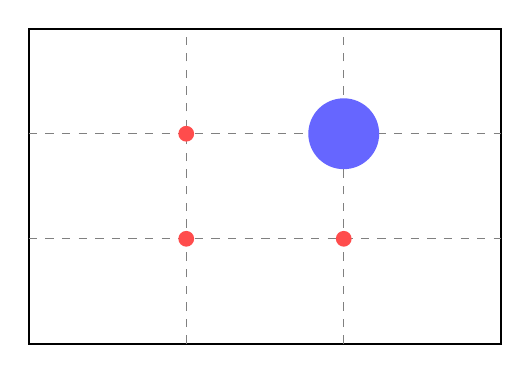
\begin{tikzpicture}
\draw[thick] (0,0) rectangle (6,4);
\draw[gray,dashed] (2,0) -- (2,4);
\draw[gray,dashed] (4,0) -- (4,4);
\draw[gray,dashed] (0,1.333) -- (6,1.333);
\draw[gray,dashed] (0,2.667) -- (6,2.667);
\foreach \x/\y in {2/1.333,4/1.333,2/2.667,4/2.667}{\fill[red!70] (\x,\y) circle(0.1);}
\fill[blue!60] (4,2.667) circle(0.45);
\end{tikzpicture}
\caption{La règle des tiers : le sujet est placé sur une intersection.}
\end{figure}

\subsection{La section d'or}

La \terme{section d'or} est un rapport proportionnel d'environ 1,618 entre le grand et le petit côté d'une division. On l'utilise pour découper un format en deux zones dont le rapport est harmonieux : la grande zone est à la petite ce que le tout est à la grande. En pratique, on peut en approcher l'effet avec un partage à environ 62 \% et 38 \%. Son efficacité est discutée, mais elle reste un outil de proportion apprécié.

\subsection{Les grilles de colonnes et les grilles modulaires}

\begin{table}[h!]
\centering
\begin{tabular}{@{}p{3.5cm}p{5cm}p{5.5cm}@{}}
\toprule
\textbf{Type de grille} & \textbf{Principe} & \textbf{Usage courant} \\
\midrule
À colonnes & Page divisée en colonnes verticales & Journaux, magazines, sites web \\
Modulaire & Colonnes et lignes formant des modules & Catalogues, interfaces, affiches complexes \\
Hiérarchique & Zones de tailles variables selon le contenu & Pages d'accueil, mises en page libres \\
\bottomrule
\end{tabular}
\caption{Les principaux types de grilles.}
\end{table}

\begin{figure}[ht]
\centering
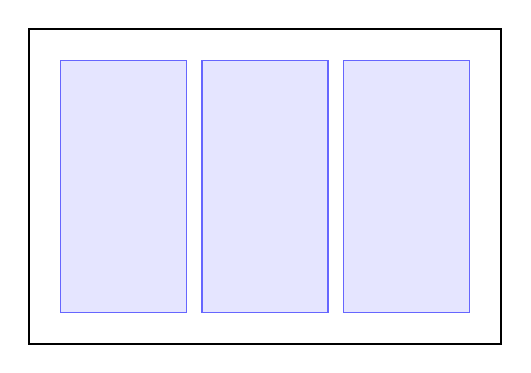
\begin{tikzpicture}
\draw[thick] (0,0) rectangle (6,4);
\foreach \x in {0.4,2.2,4.0}{\draw[blue!60,fill=blue!10] (\x,0.4) rectangle (\x+1.6,3.6);}
\end{tikzpicture}
\caption{Une grille à trois colonnes avec gouttières et marges.}
\end{figure}

\subsection{Les éléments d'une grille}

Une grille se compose de \terme{marges} (espaces autour de la page), de \terme{colonnes}, de \terme{gouttières} (espaces entre colonnes) et parfois de \terme{lignes de base} sur lesquelles s'alignent les lignes de texte.

\subsection{Étude de cas : l'école suisse et Josef Müller-Brockmann}

Le graphiste suisse Josef Müller-Brockmann (1914-1996) a fait de la grille un principe central de sa pratique, notamment dans ses affiches pour les concerts de la Tonhalle de Zurich. Il a aussi publié \anglais{Grid Systems in Graphic Design} (1981), ouvrage de référence sur le sujet. Le style international ou « suisse » repose sur des grilles rigoureuses, des textes alignés à gauche et une typographie sans empattement.

\begin{astuce}
Dans \logiciel{Illustrator}, crée des repères à partir de rectangles (Affichage, Repères, Créer des repères). Dans \logiciel{Photoshop}, utilise Affichage, Nouvelle disposition de repères pour générer colonnes et marges.
\end{astuce}

\begin{retenir}
\begin{itemize}
  \item Une grille organise le placement des éléments et assure la cohérence.
  \item La règle des tiers et la section d'or sont des aides de proportion.
  \item Les grilles se composent de marges, colonnes, gouttières et lignes de base.
\end{itemize}
\end{retenir}

%==================================================
\section{Les erreurs courantes de composition}

\subsection{Tableau des erreurs}

\begin{table}[h!]
\centering
\begin{tabular}{@{}p{3.5cm}p{4.8cm}p{5.7cm}@{}}
\toprule
\textbf{Erreur} & \textbf{Symptôme} & \textbf{Correction} \\
\midrule
Surcharge & Trop d'éléments, aucun espace & Supprimer, prioriser, aérer \\
Hiérarchie plate & Tout a la même importance & Définir trois niveaux, jouer sur taille et contraste \\
Alignements approximatifs & Éléments presque alignés & Utiliser repères et outils d'alignement \\
Espaces incohérents & Marges et espacements variables & Définir une échelle d'espaces et la respecter \\
Contraste insuffisant & Texte difficile à lire & Augmenter l'écart de valeur \\
Trop de styles & Polices, couleurs et effets multiples & Limiter à un petit système cohérent \\
Centrage systématique & Monotonie, rigidité & Essayer l'asymétrie et l'alignement à gauche \\
Effets gratuits & Ombres, dégradés, contours sans fonction & Ne garder que ce qui sert le message \\
\bottomrule
\end{tabular}
\caption{Les erreurs courantes de composition et leur correction.}
\end{table}

\subsection{Une méthode de vérification}

\begin{enumerate}
  \item \terme{Squint test} : floute ou réduis la composition ; la hiérarchie doit rester visible.
  \item \terme{Test des niveaux de gris} : vérifie les contrastes de valeur.
  \item \terme{Test de suppression} : retire un élément ; si rien ne manque, supprime-le.
  \item \terme{Test des alignements} : affiche les repères et vérifie les axes.
  \item \terme{Regard neuf} : éloigne-toi ou reviens plus tard sur la composition.
\end{enumerate}

\begin{erreur}
Corriger une composition en lui ajoutant de nouveaux éléments : la plupart des problèmes se règlent en retirant, en alignant ou en espaçant.
\end{erreur}

\begin{retenir}
\begin{itemize}
  \item Les erreurs fréquentes viennent de la surcharge, d'une hiérarchie floue et d'alignements approximatifs.
  \item Une méthode de vérification simple (flou, niveaux de gris, suppression) suffit à les repérer.
\end{itemize}
\end{retenir}

%==================================================
\section*{Exercices pratiques}
\addcontentsline{toc}{section}{Exercices pratiques}

\subsubsection*{Exercice 1 --- Recomposer une affiche selon la règle des tiers (\logiciel{Photoshop})}

Choisis une photographie dont le sujet est centré. Dans \logiciel{Photoshop}, affiche une disposition de repères en tiers, puis recadre l'image pour placer le sujet sur une intersection. Ajoute un titre aligné sur une ligne de tiers.

\textbf{Critère de réussite :} le sujet occupe une intersection, le titre est lisible et aligné, et la composition semble plus dynamique que l'originale.

\subsubsection*{Exercice 2 --- Hiérarchie sur un flyer (\logiciel{Illustrator})}

Crée un flyer A5 pour un événement fictif contenant un titre, un sous-titre, trois informations pratiques et un logo. Définis trois niveaux de hiérarchie en jouant sur la taille, la graisse et le contraste.

\textbf{Critère de réussite :} en plissant les yeux, on lit dans l'ordre le titre, le sous-titre, puis les informations pratiques ; la version en niveaux de gris reste lisible.

\subsubsection*{Exercice 3 --- Grille à trois colonnes (\logiciel{Illustrator})}

Construis une page de magazine avec une grille à trois colonnes, des marges de 15~mm et des gouttières de 5~mm. Place un titre, deux blocs de texte et une image, tous alignés sur la grille.

\textbf{Critère de réussite :} tous les éléments s'appuient sur les colonnes et les marges, et les espaces entre blocs sont plus grands que ceux à l'intérieur des blocs.

%==================================================
\section*{Conclusion du chapitre}
\addcontentsline{toc}{section}{Conclusion du chapitre}

Dans ce chapitre, nous avons parcouru les fondements de la composition graphique : sa définition, les éléments du langage visuel, l'équilibre, la hiérarchie, l'alignement, le contraste, la proximité, la répétition et le rythme, l'espace négatif, les grilles et les erreurs courantes.

\begin{itemize}
  \item La composition est une organisation intentionnelle au service d'un message.
  \item Elle s'appuie sur des principes qui se combinent plus qu'ils ne s'opposent.
  \item Elle se vérifie par des tests simples et se perfectionne par la pratique.
\end{itemize}

Ces principes sont indépendants des logiciels : tu les retrouveras dans chaque projet. Dans le chapitre suivant, nous étudions la couleur, un autre élément essentiel du langage visuel.

\vspace{1em}

\begin{center}
\textbf{Prochain chapitre : Chapitre 3 --- Théorie des couleurs.}
\end{center}
